\documentclass{beamer}

\usepackage[utf8]{inputenc}
\usepackage{default}

\usetheme{Warsaw}

\begin{document}

\begin{frame}
 
 \frametitle{Numbers are incomplete without units} \pause
 
 \begin{itemize}
  
  \item  Apart from being a constant quantity, a number usually makes sense when presented along with units. \pause
  
    \begin{figure}
    \centering
    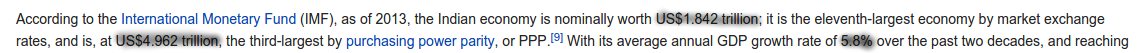
\includegraphics[width = 1.0\textwidth]{images/ex_6}
  \end{figure}
  \pause 
  \item Units help in improving recall.  \pause
  
  \begin{itemize}
      \item In above example 1.842 as number alone would not match with the fact regarding economy in knowledge base. \pause
      \item But with the unit trillion USD, we can normalize the value and then it would match exisiting facts in knowledge base. 
      
  \end{itemize}
  \end{itemize}
  \end{frame}
  
  \begin{frame}
  \frametitle{Numbers are in
\begin{frame}
 
 \frametitle{Numbers are incomplete without units} \pause
 
 \begin{itemize}
  
  \item  Apart from being a constant quantity, a number usually makes sense when presented along with units. \pause
  
    \begin{figure}
    \centering
    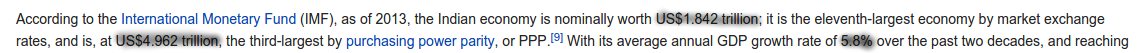
\includegraphics[width = 1.0\textwidth]{images/ex_6}
  \end{figure}
  \pause 
  \item Units help in improving recall.  \pause
  
  \begin{itemize}
      \item In above example 1.842 as number alone would not match with the fact regarding economy in knowledge base. \pause
      \item But with the unit trillion USD, we can normalize the value and then it would match exisiting facts in knowledge base. 
      
  \end{itemize}
  \end{itemize}
  \end{frame}
  
  \begin{frame}
  \frametitle{Numbers are incomplete without units} 
    \begin{figure}
    \centering
    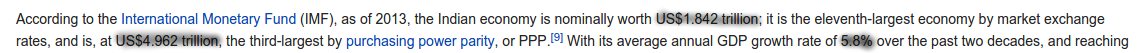
\includegraphics[width = 1.0\textwidth]{images/ex_6}
  \end{figure}
  
  \begin{itemize}
  \item Units help in reducing false positives and hence improving precision. \pause
  \begin{itemize}
      \item If there is a fact, e.g, \textbf{inflation(India, 1.842\%)} in knowledge base, then ignoring units can cause an incorrect match which leads in learning towards noisy patterns.
  \end{itemize}
  
 \end{itemize}

 
\end{frame}

\begin{frame}
 \frametitle{Unit Extraction is not easy!} \pause
 
 \begin{itemize}
    \item Different ways to represent a single unit. \pause
    
    \begin{itemize}
     \item Tunisia occupies an area of 163,610 \textbf{square kilometres}, of which 8,250 are water. \pause
     \item With an area of about 9.6 \textbf{million $km^{2}$}, the People's Republic of China is the 3rd largest country in total area behind Russia and Canada, and very similar to the United States.
    \end{itemize}
\pause
    
    \item Multiple units to represent a single numerical fact. \pause
    \begin{itemize}
      \item Vatican City, a walled enclave within the city of Rome, with an area of approximately \textbf{44 hectares} \textbf{(110 acres)}, and a population of 842, is the smallest internationally recognized independent state in the world by both area and population.
    \end{itemize}
 \end{itemize}
\end{frame}


\begin{frame}
 \frametitle{Overview of Unit Extraction System} \pause
 
 \begin{itemize}
  
  \item A discriminative context free grammmar with scores
attached to each possible production in the grammar. \pause
  \item A production P in the grammar is of the form  $ R ::= R_{1} R_{2}$ , scored as 
\begin{equation*}
	score(P) = \textbf{w . f}(P, x, i, j, k), 
\end{equation*}
where $(i,j)$ and $(j+1,k)$ are text spans in $x$ that $R_{1}$ and $R_{2}$
cover.
 \end{itemize}
\end{frame}

\begin{frame}
 \frametitle{Overview of Unit Extraction System}
 \begin{itemize}
  \item Some of the features that grammar uses to assign the best scores to various
parses are as belows: \pause
    \begin{itemize}
        \item Matches with Unit Catalog \pause
	\item Lexical Clues \pause
	\item Relative Frequency - Prior of the word to be present as unit, then as an
	  non-unit word. This is derived from WordNet ontologies. \pause
	\item Co-occurrence statistics - presence of strongly co-occuring words in the
	  text can help in disambiguating the various candidate units 
    \end{itemize}
 \end{itemize}

 
 
\end{frame}

complete without units} 
    \begin{figure}
    \centering
    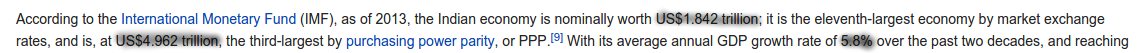
\includegraphics[width = 1.0\textwidth]{images/ex_6}
  \end{figure}
  
  \begin{itemize}
  \item Units help in reducing false positives and hence improving precision. \pause
  \begin{itemize}
      \item If there is a fact, e.g, \textbf{inflation(India, 1.842\%)} in knowledge base, then ignoring units can cause an incorrect match which leads in learning towards noisy patterns.
  \end{itemize}
  
 \end{itemize}

 
\end{frame}

\begin{frame}
 \frametitle{Unit Extraction is not easy!} \pause
 
 \begin{itemize}
    \item Different ways to represent a single unit. \pause
    
    \begin{itemize}
     \item Tunisia occupies an area of 163,610 \textbf{square kilometres}, of which 8,250 are water. \pause
     \item With an area of about 9.6 \textbf{million $km^{2}$}, the People's Republic of China is the 3rd largest country in total area behind Russia and Canada, and very similar to the United States.
    \end{itemize}
\pause
    
    \item Multiple units to represent a single numerical fact. \pause
    \begin{itemize}
      \item Vatican City, a walled enclave within the city of Rome, with an area of approximately \textbf{44 hectares} \textbf{(110 acres)}, and a population of 842, is the smallest internationally recognized independent state in the world by both area and population.
    \end{itemize}
 \end{itemize}
\end{frame}


\begin{frame}
 \frametitle{Overview of Unit Extraction System} \pause
 
 \begin{itemize}
  
  \item A discriminative context free grammmar with scores
attached to each possible production in the grammar. \pause
  \item A production P in the grammar is of the form  $ R ::= R_{1} R_{2}$ , scored as 
\begin{equation*}
	score(P) = \textbf{w . f}(P, x, i, j, k), 
\end{equation*}
where $(i,j)$ and $(j+1,k)$ are text spans in $x$ that $R_{1}$ and $R_{2}$
cover.
 \end{itemize}
\end{frame}

\begin{frame}
 \frametitle{Overview of Unit Extraction System}
 \begin{itemize}
  \item Some of the features that grammar uses to assign the best scores to various
parses are as belows: \pause
    \begin{itemize}
        \item Matches with Unit Catalog \pause
	\item Lexical Clues \pause
	\item Relative Frequency - Prior of the word to be present as unit, then as an
	  non-unit word. This is derived from WordNet ontologies. \pause
	\item Co-occurrence statistics - presence of strongly co-occuring words in the
	  text can help in disambiguating the various candidate units 
    \end{itemize}
 \end{itemize}

 
 
\end{frame}





\end{document}
